\chapter{CH$_{3}$NH$_{2}$ survey in low mass star-forming regions
\label{chap:appendixA}}

低質量星形成領域は彗星の起源とより関係していると考えられるため、これらの領域でのメチルアミンサーベイも意義がある。Orion-KLだけでなく次の2天体でもサーベイを行ったが、いずれの天体でもメチルアミンは検出できなかった。そこでノイズの強度を用いて柱密度の上限を計算し制限を設けた。その結果を報告する。

We also 

\section{IRAS 16293}
IRAS 16293は二つの星からなる連星系で、そのうちsource Bは線幅が狭くラインサーベイに適している。この天体でのCH$_{3}$NH$_{2}$サーベイは過去行われているが、検出不可を報告していた。その論文はband 7の探査であり、source Bの1ピクセルから取得したスペクトルを使って解析をしていた。そこで我々は他の周波数帯で空間バイアスをかけずに追解析を行った。ラインサーベイの手法は2.2.2章と同じものである。

\subsection{Observation data}
PILSサーベイのうちBand 6のアーカイブデータを使用した。データキャリブレーションはOya+2018(?)で行われていた。以下に観測諸元を示す。


\subsection{Results}
観測周波数内には


\begin{figure}[H]
  \centering
  \includegraphics[width=0.7\textwidth]{LMSFR/IRAS16293_mom0.eps}
  \caption{Integrated intensity map around 247.362 GHz. The white contours represent the 1.3 mm continuum map, where the contour levels are 10 \%, 30 \%, 50 \%, 70 \%, 90 \% of the peak intensity.}
  \label{IRAS16293_mom0}
\end{figure}

\begin{figure}[H]
  \centering
  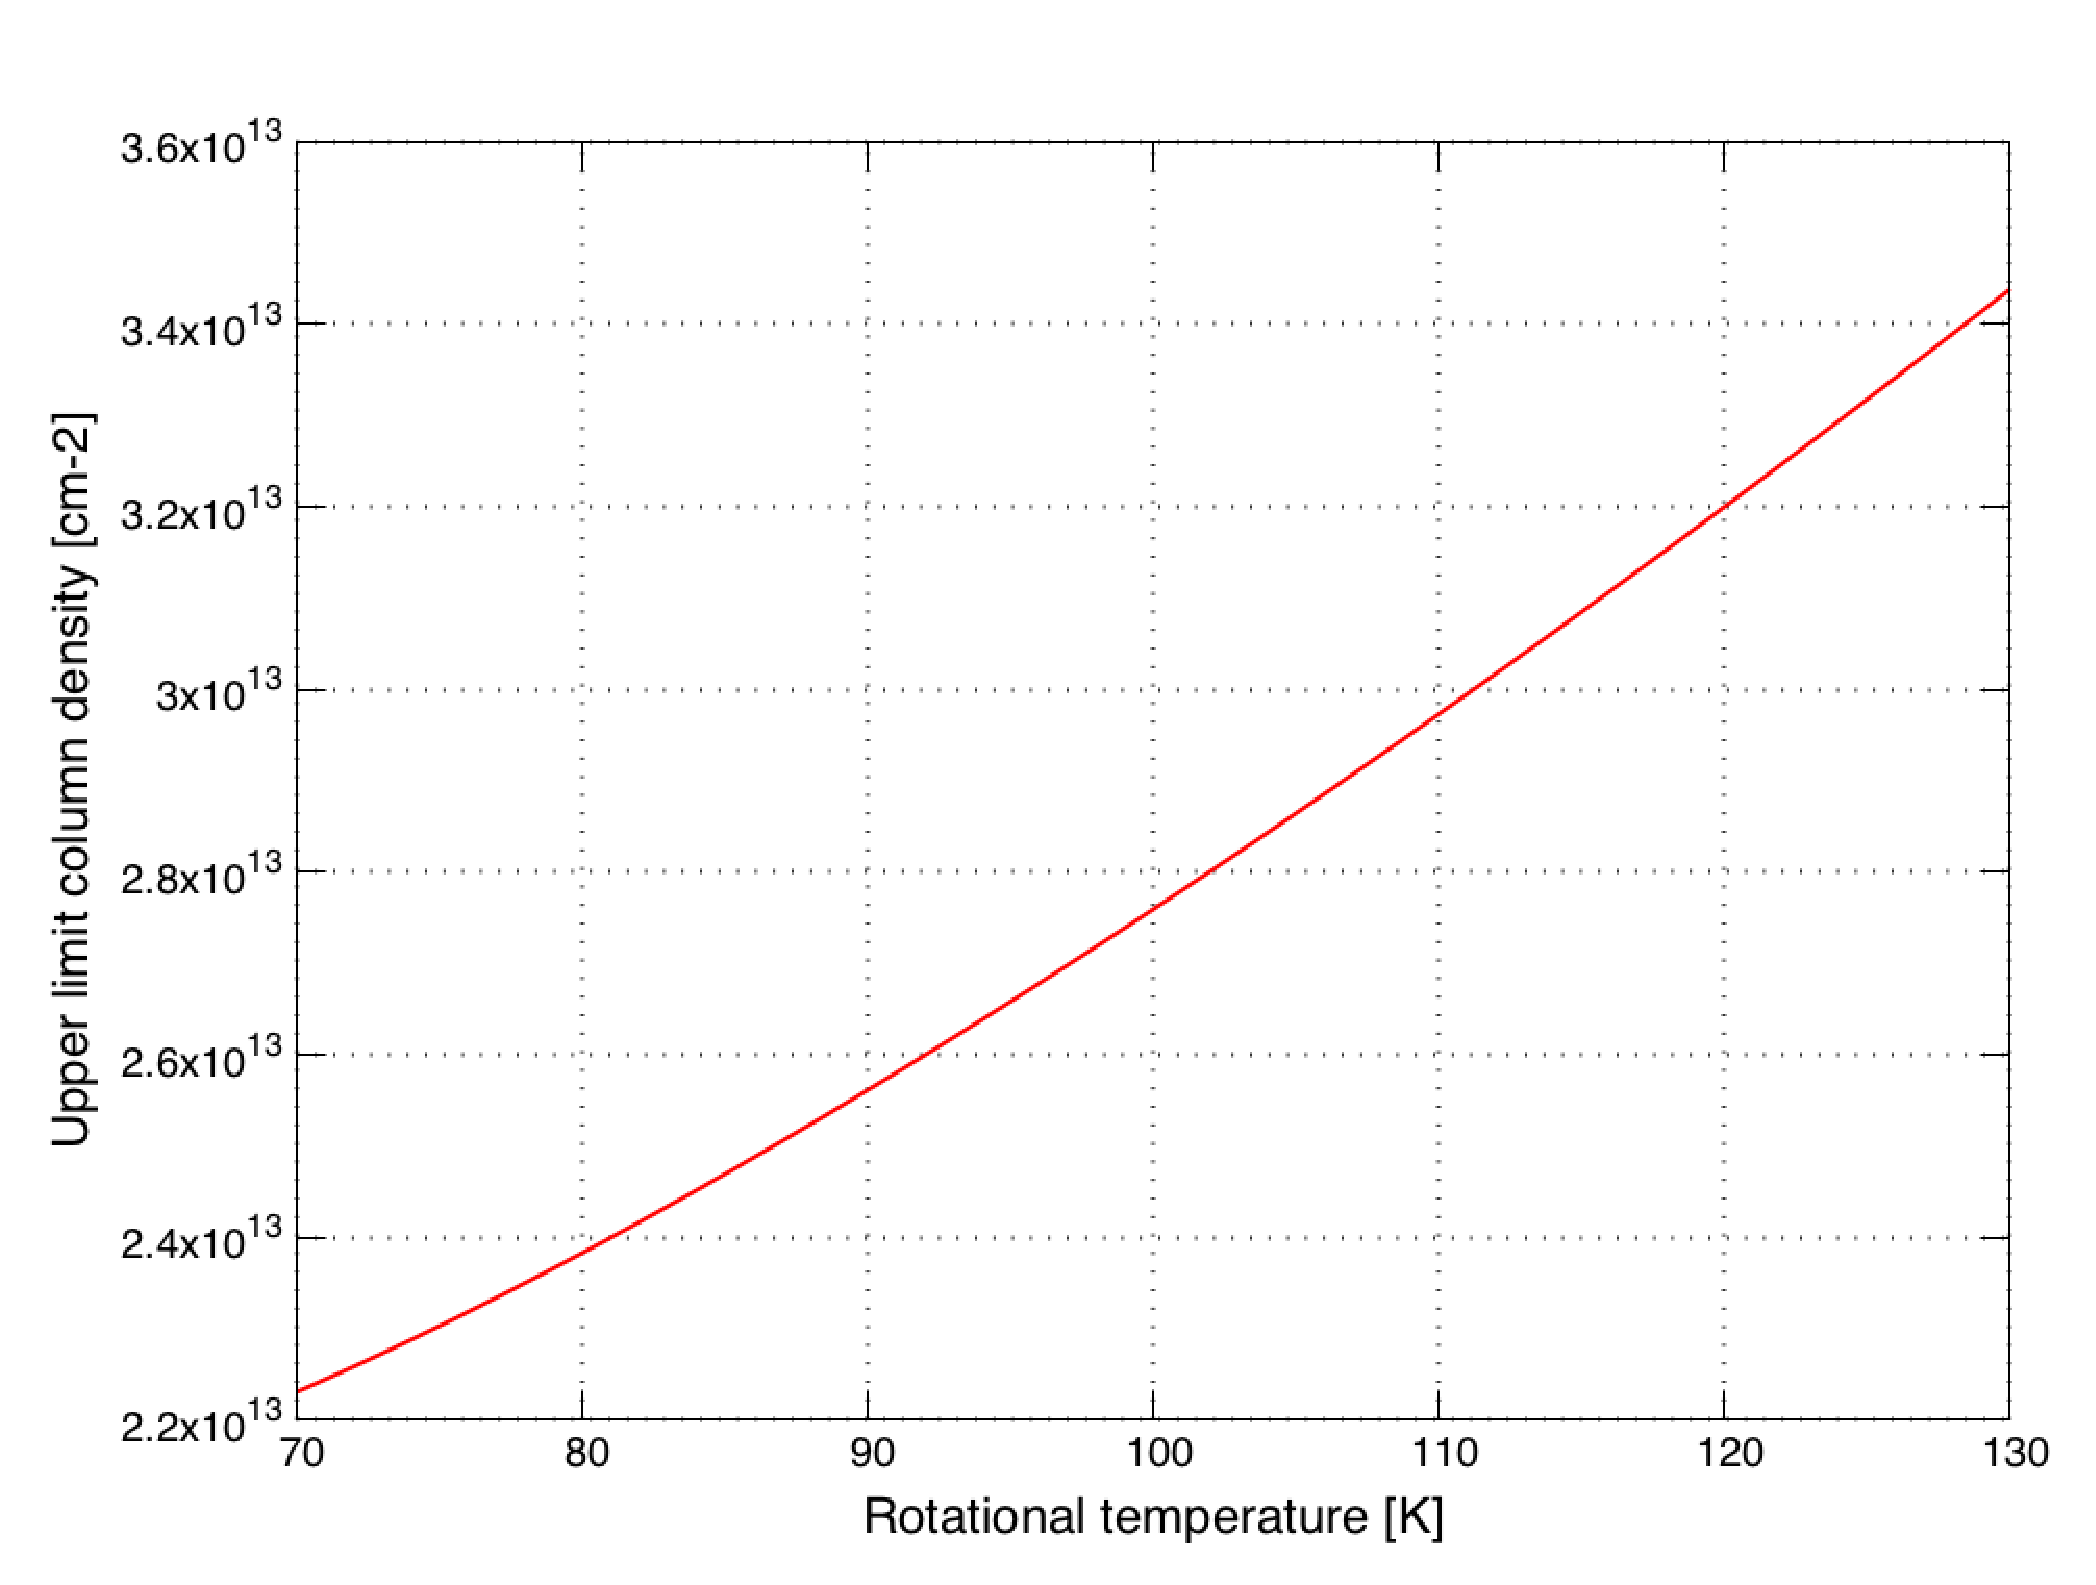
\includegraphics[width=0.7\textwidth]{LMSFR/IRAS16293.eps}
  \caption{Upper limit column density for the strongest CH$_{3}$NH$_{2}$ transition
  ($7_{2}E_{1-1} \rightarrow 7_{1}E_{1-1}$) as function of T$_{\textrm{rot}}$. A 3$\sigma$ value of 
  11.4 mJy beam$^{-1}$ is used.}
  \label{IRAS16293_MA}
\end{figure}



\section{L483}
\subsection{Observation data}
\subsection{Results}

\begin{figure}[H]
  \centering
  \includegraphics[width=0.7\textwidth]{LMSFR/L483_mom0.eps}
  \caption{Integrated intensity map around 217.079 GHz. The white contours represent the 1.3 mm continuum map, where the contour levels are 10 \%, 30 \%, 50 \%, 70 \%, 90 \% of the peak intensity.}
  \label{L483_mom0}
\end{figure}

\begin{figure}[H]
  \centering
  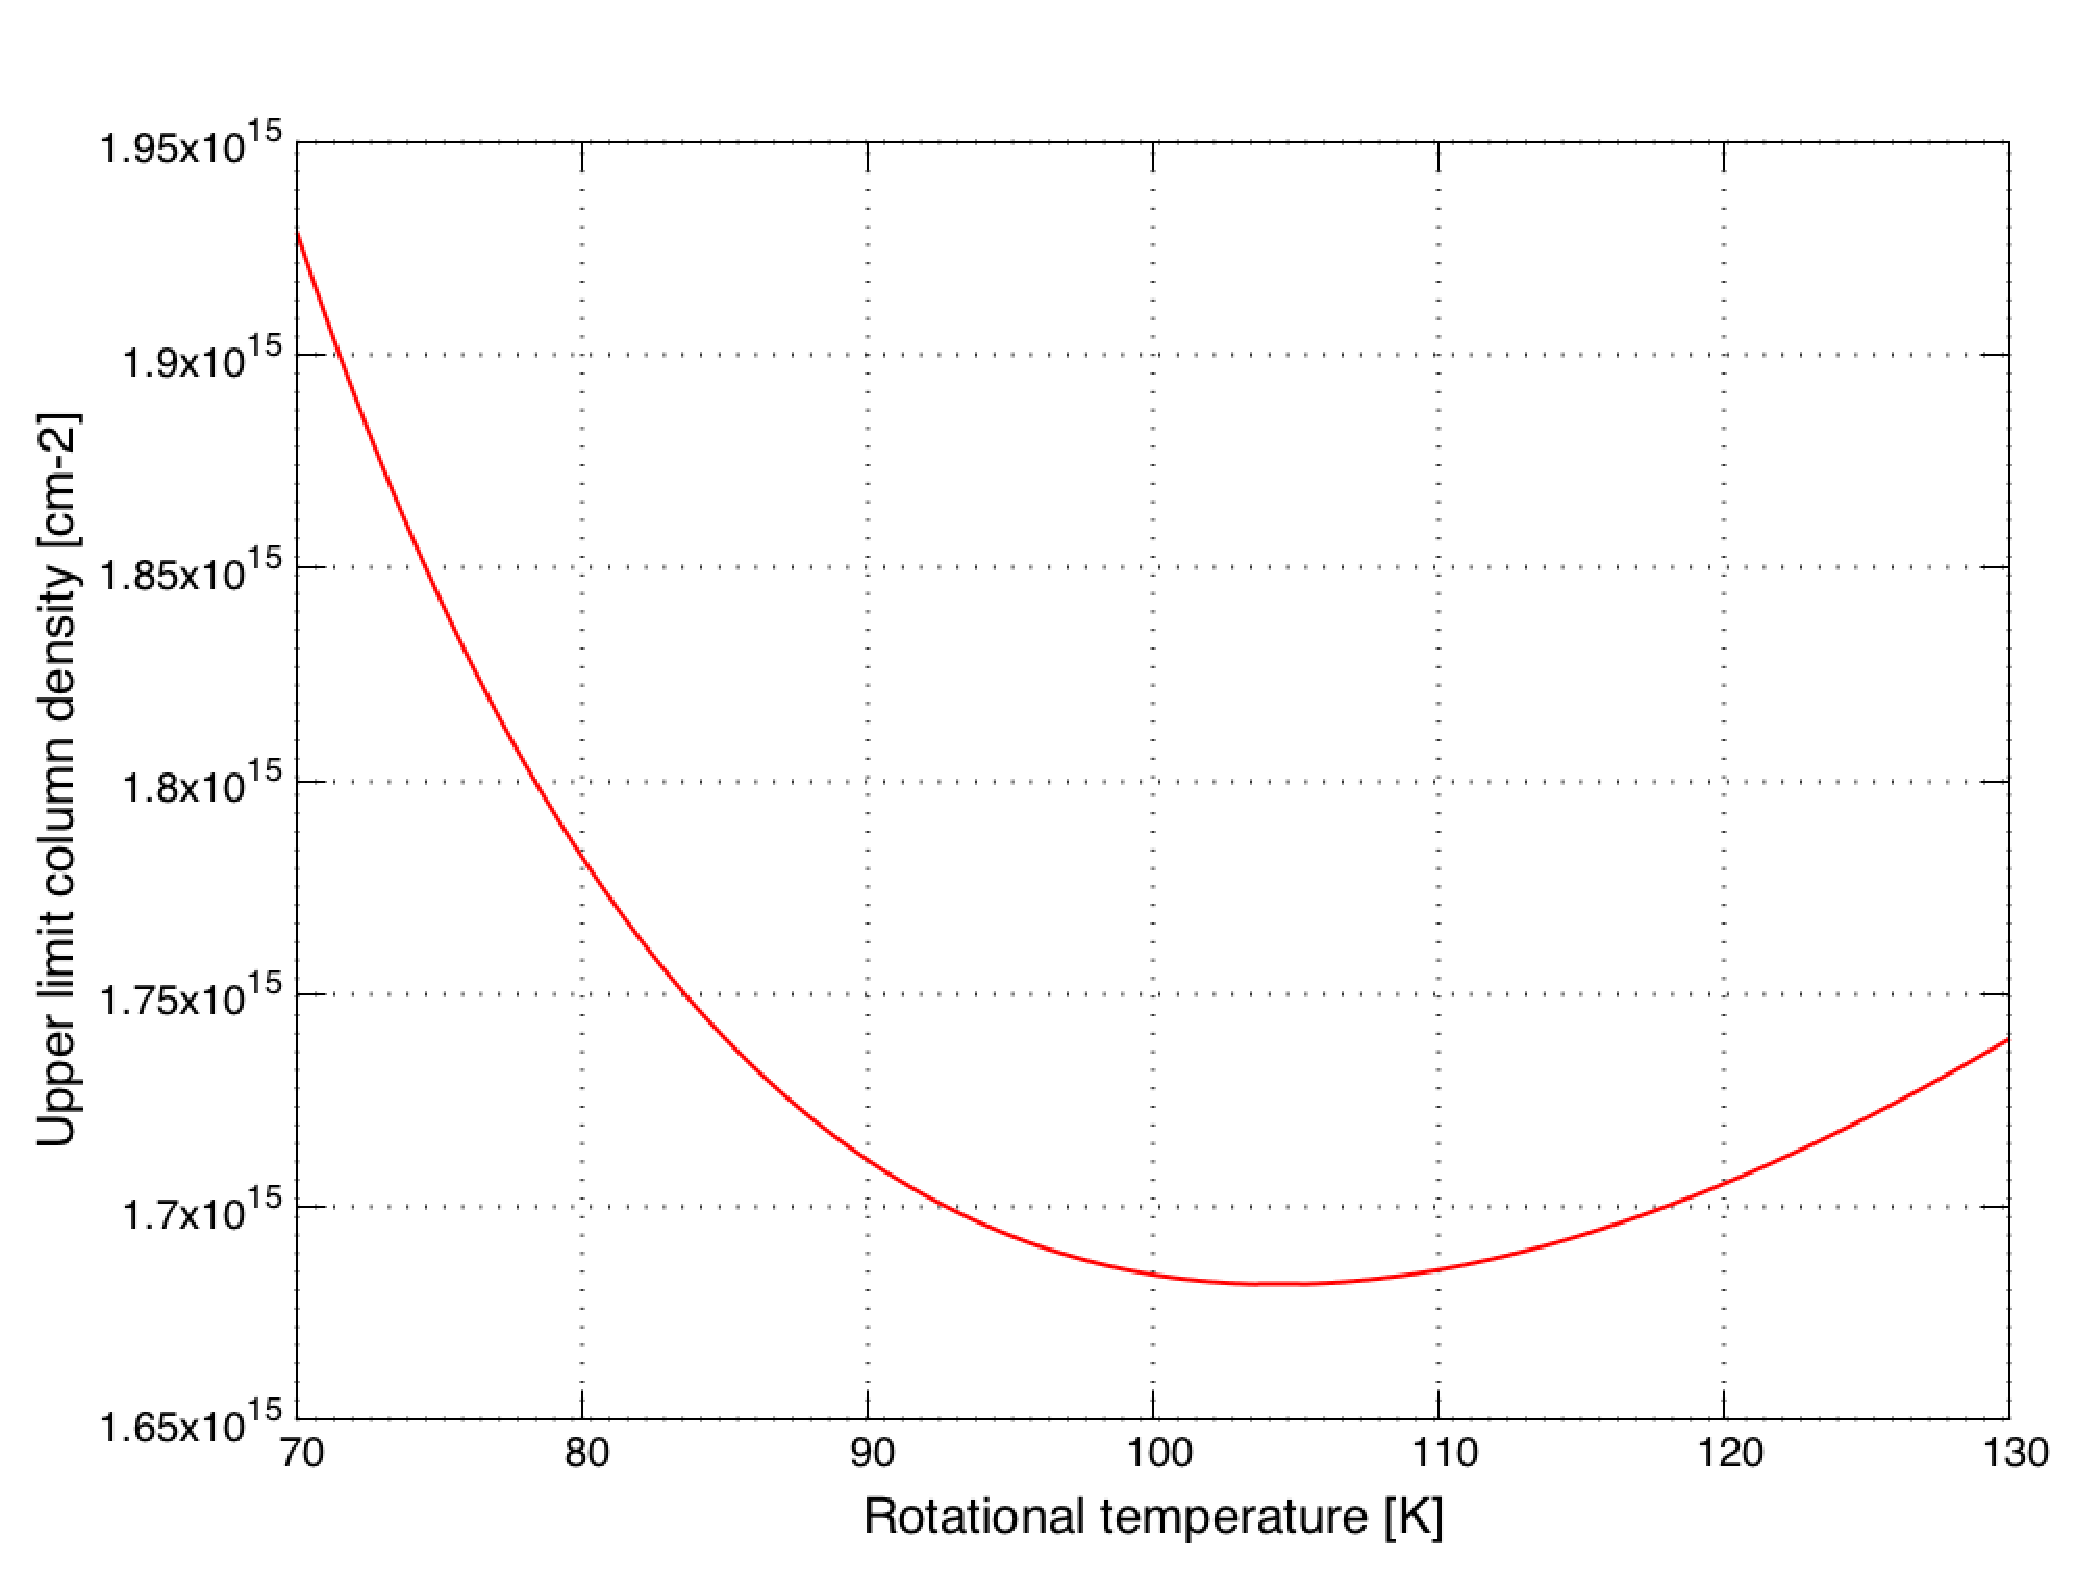
\includegraphics[width=0.7\textwidth]{LMSFR/L483.eps}
  \caption{Upper limit column density for the strongest CH$_{3}$NH$_{2}$ transition
  ($11_{2}A_{1} \rightarrow 11_{2}A_{2}$) as function of T$_{\textrm{rot}}$. A 3$\sigma$ value of 
  22.5 mJy beam$^{-1}$ is used.}
  \label{L483_MA}
\end{figure}

